%%=============================================================================
%% Inleiding
%%=============================================================================

\chapter{\IfLanguageName{dutch}{Inleiding}{Introduction}}
\label{ch:inleiding}

%%De inleiding moet de lezer net genoeg informatie verschaffen om het onderwerp te begrijpen en in te zien waarom de onderzoeksvraag de moeite waard is om te onderzoeken. In de inleiding ga je literatuurverwijzingen beperken, zodat de tekst vlot leesbaar blijft. Je kan de inleiding verder onderverdelen in secties als dit de tekst verduidelijkt. Zaken die aan bod kunnen komen in de inleiding~\autocite{Pollefliet2011}:

%%\begin{itemize}
  %%\item context, achtergrond
  %%\item afbakenen van het onderwerp
  %%\item verantwoording van het onderwerp, methodologie
  %%\item probleemstelling
  %%\item onderzoeksdoelstelling
  %%\item onderzoeksvraag
  %%\item \ldots
%%\end{itemize}

Het geautomatiseerd parsen van systeem logs klinkt als een complexe casus en uit de titel kan het probleemdomein niet onmiddellijk afgeleid worden. Om deze titel en aldus het onderwerp beter te begrijpen moet er ten eerste begrepen worden binnen welke context het parsen van systeem logs plaatsvindt. Voordat het domein zal toegelicht worden is het handig om eerst nog toe te lichten wat systeem logs specifiek zijn. Hierover geeft de eerste sectie meer informatie. Een tweede onderwerp, dat cruciaal is binnen dit onderzoek, is wat het parsen van logs specifiek inhoudt. Hierop wordt dieper ingegaan in de tweede sectie. Een belangrijk begrip bij het parsen van logs is `reguliere expressies`, reguliere expressies worden binnen applicatieontwikkeling veel gebruikt en zijn ook een zeer belangrijk onderdeel bij het parsen van logs. De derde sectie zal dit begrip verder bespreken. In de laatste sectie wordt er dieper ingegaan op het specifieke domein waarop toegespitst wordt binnen deze bachelorproef. 

\section{Wat is een log?}

Een systeem log is een log file gelinkt aan een bepaald systeem (zoals bv. Windows, Linux, etc.). Een log file is een primaire data bron voor observaties. Het is een datafile gegenereerd door een computer die informatie bevat over gebruikpatronen, activiteiten en operaties die plaatsvinden binnen een besturingssysteem, een applicatie, een server of een apparaat. Log files worden gegenereerd wanneer specifieke handelingen gebeuren over het netwerk of binnen de applicatie. Organisaties binnen de IT sector gebruiken logfiles om het gebruik en de activiteiten van hun gebruikers te analyseren en ook om het gedrag van de applicatie vast te leggen of om fouten te detecteren. De hoofdreden waarom log files bestaan is dat ontwikkelaars van soft- en hardware het makkelijker vinden om via tekstuele data de werking van het systeem te volgen en vast te leggen. Voor elk domein binnen IT zijn er verschillende logs, voor security, servers, applicaties, etc.\\

In figuur \ref{pic:loglijnen} wordt een voorbeeld weergegeven van enkele loglijnen binnen een log bestand dat benut zal worden binnen dit onderzoek.

\begin{figure}[!htp]
    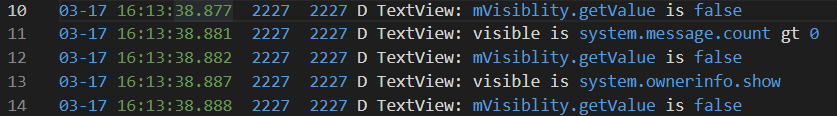
\includegraphics{log_lijnen.png}
    \caption{Voorbeeld van een aantal lijnen uit een log bestand.}
    \label{pic:loglijnen}
\end{figure}

\section{Log Parsing}

Log parsing is een methode die wordt toegepast bij het analyseren van logfiles. Voordat een logfile kan geanalyseerd worden moet eerst de logfile opgedeeld worden in verschillende delen met specifieke labels. Dit is waarvoor parsers worden gebruikt. Log parsing is vooral belangrijk om een logfile goed te kunnen analyseren want door logparsing toe te passen kan er specifieke data uit de logs, zoals tijdstip, hostnaam, service naam, etc., makkelijk afgeleid worden. Log parsing kan op verschillende manieren gebeuren. Om loglijnen op te delen in stukken die makkelijker te analyseren zijn, worden meestal reguliere expressies gebruikt. Reguliere expressies zijn een opeenvolging van symbolen en karakters die een string of patroon waarnaar gezocht wordt binnen een tekst voorstellen (zie sectie \ref{section:reguliereexpressie}).

Log parsing methodes worden toegepast op verschillende manieren met verschillende strategieën. Deze strategieën ondersteunen de toepassing van de methodologieën. Hieronder worden de meest voorkomende strategieën binnen het onderzoek van deze bachelorproef toegelicht:
\begin{itemize}
    \item Frequent pattern mining: Deze techniek is gebaseerd op frequente patronen die vaak voorkomen in bepaalde datasets.
    Zo kunnen bijvoorbeeld events in een log gezien worden als constante tokens die vaak voorkomen. De procedure die hiermee gepaard gaat is als volgt:
    \begin{enumerate}
        \item De log data meerdere keren overlopen.
        \item Opbouwen van frequente items en patronen bij elke iteratie.
        \item Groeperen van log messages in verschillende clusters.
        \item Het extraharen van event templates bij elke cluster. 
    \end{enumerate}

    \item Clustering: Bepaalde loglijnen kunnen voldoen aan eenzelfde opbouw of `template`. Deze loglijnen hebben een gelijkaardige vorm. Uit log files kunnen meerdere vormen gehaald worden en deze definiëren in een beperkt aantal clusters. Elke loglijn wordt onderzocht en als deze voldoet aan het template van één van deze clusters dan wordt de loglijn toegevoegd aan deze cluster. Zo niet, dan wordt op basis van de loglijn een nieuwe cluster aangemaakt.\\
    
    \item Heuristieken: Loglijnen hebben unieke karakteristieken waardoor er heuristieken kunnen toegepast worden binnen de logparsing. Dit kan op verschillende manieren:
    \begin{enumerate}
        \item Het verdelen in meerdere groepen van loglijnen op basis van het aantal voorkomens van constante en variabele tokens.
        \item Door te verdelen op basis van de lengte van de log messages, de token positie, i.e.\ waar in de log de message plaatsvindt, en mapping relaties.
        \item Met een diepte-gelimiteerde boom de relaties vastleggen en partitioneren.
    \end{enumerate}

\end{itemize}
Andere strategieën bestaan nog maar worden later verder in detail besproken in hoofdstuk \ref{ch:stand-van-zaken}. Voor een referentie naar de verschillende methodes zie tabel \ref{table:parserssamenvatting}.

\section{Reguliere Expressie}
\label{section:reguliereexpressie}
De informatie binnen deze sectie is gebaseerd op een online artikel \autocite{regexwebsite}.

Binnen de log parsing methodes die zullen behandeld worden in dit onderzoek zullen reguliere expressies regelmatig aangehaald worden. Dit is omdat reguliere expressies één van de makkelijkste en meest performante manieren zijn om data op te halen uit tekstbestanden. Een reguliere expressie is een manier om patronen te beschrijven waardoor een programma verschillende soorten tekst kan herkennen. Reguliere expressies worden vooral gebruikt om bepaalde stukken uit teksten te filteren. Voorbeelden hiervan zijn: Achterhalen of een bepaalde tekst een email- of IP-adres bevat. Hierdoor wordt natuurlijk direct duidelijk waarom reguliere expressies zo krachtig zijn binnen het parsen van logs. Ze stellen ons in staat om efficiënt logs te overlopen en te zien of ze aan een bepaalde syntax voldoen. Zo worden reguliere expressies gebruikt binnen bepaalde parsers om al een eerste filtering door de log messages uit te voeren. Hieronder wordt een voorbeeld gegeven van een reguliere expressie voor het vinden van een emailadres.
\begin{verbatim}
    ^[a-zA-Z\.]+@([a-zA-Z]+\.)+[a-zA-Z]{2,4}$
\end{verbatim}

Dit voorbeeld ziet er complex uit maar de betekenis is makkelijk te achterhalen. Er wordt begonnen met een \verb!^! dit geeft het begin van de string aan. Hierna volgt \verb![a-zA-Z\.]!, hierbij wordt aangegeven dat het begint met een reeks letters, die beide grote en kleine letters kunnen zijn van \(a\) tot \(z\), en deze letterreeks kan punten bevatten, dit wordt aangegeven door de \verb!\.!. De schuine streep is nodig voor aan te geven dat het om een speciaal karakter gaat. Na het plusteken volgt de \verb!@! om aan te geven dat er een \verb!@! moet staan, dit is logisch voor een email adres. Hierna wordt weer aangegeven dat er een letter reeks met punten mogelijk is, die dan finaal gevolgd wordt door een letter reeks bestaande uit minimum 2 en maximum 4 letters, hiervoor wordt de \(\{2,4\}\) gebruikt.\\

Nog een veel voorkomende reguliere expressie binnen deze bachelorproef zal de reguliere expressie voor een IPv4 of IPv6 adres zijn. Hieronder worden respectievelijk reguliere expressies voor beide gegeven.
\begin{verbatim}
    ^[[0-9]{1,4}\.]{3}+[0-9]{1,4}$
\end{verbatim}
\begin{verbatim}
    ^[[0-9a-z]{4}\:]{7}+[0-9a-z]{4}$
\end{verbatim}
Hieruit kan afgeleid worden dat er bij IPv4 begonnen wordt met een combinatie van één tot vier cijfers van nul tot negen, aangegeven door \([0-9]\{1,4\}\), gevolgd door een punt. Deze soort sequentie komt exact drie keer voor en dan nog een laatste keer zonder punt. De reguliere expressie voor het IPv6 patroon is gelijk lopend maar hierbij is het duidelijk dat de sequentie zeven keer plaatsvindt met een dubbele punt (\(:\)). Hierbij is het ook duidelijk dat het over een hexadecimale sequentie door \([0-9a-z]\). Dit geeft aan dat het karakter uit een getal van nul tot negen of een letter van a tot z kan bestaan.

\section{Anomalie Detectie}

Anomaliedetectie is een moeilijk begrip omdat het een breed onderwerp is. In het algemeen is anomaliedetectie het vinden van patronen binnen de data van een bepaald systeem of een bepaalde applicatie die niet voldoen aan het verwachte gedrag. Deze patronen worden anomalieën genoemd \autocite{chandola2009anomaly}. Er wordt aan anomaliedetectie gedaan om applicaties en systemen zo performant en betrouwbaar mogelijk te houden. Voorbeelden hiervan zijn fraude detectie binnen bank applicaties (credit cards, etc.), indringers detectie binnen cybersecurity en zelfs binnen militaire surveillance om vijanden op te sporen \autocite{chandola2009anomaly}. 

Als er zich een bepaalde fout voordoet bij het gebruik van een systeem of applicatie dan kan dit leiden tot het verlies van gevoelige data. Een fout binnen het verkeer van een systeem kan ook een aanduiding zijn dat er een hacker het systeem is binnengedrongen \autocite{chandola2009anomaly}. Dit is de reden dat er geprobeerd wordt zo goed mogelijk fouten te voorkomen en zo vroeg mogelijk deze te detecteren. Anomaliedetectie wordt toegepast in verschillende domeinen en er zijn ook verschillende technieken ontwikkeld, sommige domein specifiek andere generiek, om aan anomaliedetectie te doen. 

Om fouten binnen een applicatie of systeem te detecteren wordt er gebruik gemaakt van logfiles. Door deze te analyseren kan er een perfect beeld verkregen worden van het voorloop van het systeem proces.

\section{\IfLanguageName{dutch}{Probleemstelling}{Problem Statement}}
\label{sec:probleemstelling}

%%Uit je probleemstelling moet duidelijk zijn dat je onderzoek een meerwaarde heeft voor een concrete doelgroep. De doelgroep moet goed gedefinieerd en afgelijnd zijn. Doelgroepen als ``bedrijven,'' ``KMO's,'' systeembeheerders, enz.~zijn nog te vaag. Als je een lijstje kan maken van de personen/organisaties die een meerwaarde zullen vinden in deze bachelorproef (dit is eigenlijk je steekproefkader), dan is dat een indicatie dat de doelgroep goed gedefinieerd is. Dit kan een enkel bedrijf zijn of zelfs één persoon (je co-promotor/opdrachtgever).

Dit onderzoek zal een meerwaarde vormen voor enkele personen. Als eerste zal de opdrachtgever van dit onderzoek een meerwaarde uit deze bachelorproef halen als informatiebron. Deze bachelorproef zal voor hem een verduidelijking betekenen binnen het onderwerp van logparsing en zal hem in staat stellen om duidelijk de juiste logparser te kiezen voor verder onderzoek binnen anomaliedetectie. Alsook zal dit onderzoek een meerwaarde vormen voor het bedrijf Exitas, dat heeft bijgedragen als co-promotor binnen deze bachelorproef. Dit bedrijf hanteert op dit moment nog een manuele manier van het parsen van systeem logs. Dit onderzoek zal hen in staat stellen om een duidelijk overzicht te bemachtigen van de huidige logparsers en hun specificaties. Ten laatste zal dit onderzoek vooral een meerwaarde zijn binnen verder onderzoek binnen het domein van anomaliedetectie en log parsing. Zo zal dit onderzoek een uitgebreide uiteenzetting geven van enkele beschikbare tools voor log parsing op dit moment. 


\section{\IfLanguageName{dutch}{Onderzoeksvraag}{Research question}}
\label{sec:onderzoeksvraag}

%%Wees zo concreet mogelijk bij het formuleren van je onderzoeksvraag. Een onderzoeksvraag is trouwens iets waar nog niemand op dit moment een antwoord heeft (voor zover je kan nagaan). Het opzoeken van bestaande informatie (bv. ``welke tools bestaan er voor deze toepassing?'') is dus geen onderzoeksvraag. Je kan de onderzoeksvraag verder specifiëren in deelvragen. Bv.~als je onderzoek gaat over performantiemetingen, dan 

Bij dit onderzoek wordt de vraag gesteld: 'Wat is de huidige snelste log parser die een duidelijke en analyseerbare parsing oplevert voor loganomaliedetectie en die ongesuperviseerd getraind kan worden in een real-time setting?'.

Een gelijkaardig onderzoek is reeds gevoerd in de paper `Tools and Benchmarks for Automated Log Parsing` \autocite{TBA2019}. Dit onderzoek is echter al 3 jaar oud en binnen het onderzoek van deze bachelorproef zal er gekeken worden naar andere beperkingen, die reeds binnen de onderzoeksvraag werden vermeld.

Het onderzoek zal ten eerste beperkt worden tot een real-time setting, omdat deze bachelorproef een basis voor de analyse en anomaliedetectie van logfiles zal vormen. Hierbij is tijd een belangrijke factor. 

Andere beperkingen die in het onderzoek zullen opgelegd worden, zijn:
\begin{itemize}
    \item Een parser moet een goede parsing opleveren, i.e.\ een leesbare en duidelijk analyseerbare parsing.
    \item Een gekozen parser moet ‘ongesuperviseerd’ kunnen getraind worden.
    \item Een parser moet snel werken. Hiermee wordt een tijdscomplexiteit bedoeld die hoogstens lineair is in het aantal karakters en aantal verschillende parserboodschappen.
\end{itemize}

\section{\IfLanguageName{dutch}{Onderzoeksdoelstelling}{Research objective}}
\label{sec:onderzoeksdoelstelling}

%%Wat is het beoogde resultaat van je bachelorproef? Wat zijn de criteria voor succes? Beschrijf die zo concreet mogelijk. Gaat het bv. om een proof-of-concept, een prototype, een verslag met aanbevelingen, een vergelijkende studie, enz.

Deze bachelorproef is in het algemeen een vergelijkende studie van de verschillende logparsers. In eerste instantie zal binnen deze bachelorproef onderzocht worden of de observaties van de paper `Tools and Benchmarks for Automated Log Parsing` \autocite{TBA2019} nog steeds van toepassing zijn. Hieropvolgend zullen de 13 log parsers van de voorgenoemde paper doorgenomen worden met nieuwe datasets. Als laatste stap zullen er extra logparsers toegevoegd worden aan het onderzoek die niet reeds gedefinieerd zijn in de voorgenoemde paper. Hieruit zal blijken of Drain, i.e.\ de logparser die in de paper `Tools and Benchmarks for Automated Log Parsing` \autocite{TBA2019} naar bovenkwam als de `beste` en meest efficiënte logparser, ook binnen deze beperkingen en binnen dit onderzoek zal naar bovenkomen als de optimale keuze of dat een andere logparser er bovenuit steekt. Deze bachelorproef zal bij het onderzoek ook duidelijk weergeven hoe er gebruik gemaakt is van de logparser repository \autocite{TBA2019} zodat dit gereproduceerd kan worden. 

\section{\IfLanguageName{dutch}{Opzet van deze bachelorproef}{Structure of this bachelor thesis}}
\label{sec:opzet-bachelorproef}

% Het is gebruikelijk aan het einde van de inleiding een overzicht te
% geven van de opbouw van de rest van de tekst. Deze sectie bevat al een aanzet
% die je kan aanvullen/aanpassen in functie van je eigen tekst.

De rest van deze bachelorproef is als volgt opgebouwd:

In Hoofdstuk~\ref{ch:stand-van-zaken} wordt een overzicht gegeven van de stand van zaken binnen het onderzoeksdomein, op basis van een literatuurstudie. Hierbij wordt elke parser apart bekeken en wordt er uitgebreid ingegaan op de werking hiervan. Hiernaast zal ook nog een samenvattend overzicht weergegeven worden van alle parsers.

In Hoofdstuk~\ref{ch:methodologie} wordt de methodologie van het onderzoek toegelicht. Hierbij wordt de opzetting van het onderzoek in detail besproken zodat de werking duidelijk is voor eventueel opvolgend onderzoek. Hiernaast worden de resultaten besproken van het onderzoek. Er wordt hierbij gekeken naar de gespecifieerde vergelijkingscriteria. Ten slotte eindigt dit hoofdstuk met een toepassing van een nieuwe technologie voor het verder testen en verbeteren van parsing en met het toepassen van nieuwe datasets op de parsers die het best naar voor komen binnen het onderzoek.

In Hoofdstuk~\ref{ch:conclusie}, wordt de conclusie van het onderzoek weergegeven. Hierbij zal de parser die de beste en meest consistente resultaten behaalt naar voor komen en zullen de verwachtingen tegenover het resultaat afgewogen worden. Hiernaast worden ook nog overige vragen opgelijst tesamen met een referentie naar eventueel verdergaand onderzoek.